The performance of \acrshort{gaco} for \gls{idpcdu} is evaluated under three analyses:
\begin{itemize}
	\item Analysis of the algorithm's computational complexity.
	\item Analysis of the obtained results by the Non-parametric statistic.
	\item Analysis quality of the proposed algorithm in comparison with other algorithms.
\end{itemize}

\subsection{Analysis of the algorithm's computational complexity}
The number of times \acrshort{gaco} is iterated is denoted by $GEN\_GA$. In each iteration, the execution times of the crossover, mutation, and decoding operators are $N, p_m * N$, and $N$ times, respectively. The complexity of the algorithm is as follows:
$O($\acrshort{gaco}$)$ = $O($Pre-filtering process$)$ + $O($Initialization$)$ + $GEN\_GA\times \bigg(N \times O($Crossover$)$ + $p_{m}\times N\times O($Mutation$)$ + $N\times O($Evaluation$)$ + $O($Selection$)\bigg)$, in which the complexity of each component is as follows:
\begin{itemize}
	\item In the pre-filtering process, each edge in $G$ is traversed  one time. Therefore, the complexity of the pre-filtering process is $O(|E|)$, with $|E|$ being the number of edges in the initial graph.
	\item The initialization method needs a computational cost $O(|D|\times N)$ to generate $N$ random individuals, with $|D|$ being the number of domains.
	\item The complexity of mutation, crossover, and survival selection operators are $O(1)$, $O(|D|)$, and $O(NlogN)$, respectively.
	\item The fitness evaluation uses \gls{aco} algorithm, which starts with the initial pheromone on all edges of $G'$, so the running time of this process is $O(|E'|)$. Then, \gls{aco} performs $GEN\_ACO$ iterations over the following steps: construct solutions for $M$ ants and updates pheromone. A solution is built by Algorithm~\ref{alg:apa} with a running time of $O(|E'|\times |D|^2)$. Because each ant travels through nodes on $G'$, it constructs a list of candidate adjacent edges at every visited node. Each edge is added to the list with the running time of $O(|1|)$ of checking the $Checksum$ and $O(|D|^2)$ of the $Domain~Blacklist~Check$. Besides, every candidate list of adjacent edges has its size no more than the out-degree of the currently visited, and the total out-degree of all nodes on $G'$ is the number of edges. Update pheromone has a running time of $O(|V'|)$ because the maximum path length is the number of nodes on $G'$. Therefore, the computational complexity of the \gls{aco} algorithm is $O(ACO\;initialization)\;+\;GEN\_ACO\times M\times (O(ACO\;construct\;solutions)\;+\;O(ACO\;update\;pheromone))$, in which the complexity of \gls{aco} initialization, construct solutions, and update pheromone are $O(|E'|)$, $O(|E'|\times |D|^2)$, and $O(|V'|)$.
\end{itemize}
Therefore, $O($\acrshort{gaco}$) = $
$O(|E|) + O(|D|\times N)$ + $GEN\_GA\times\bigg(N \times O(|D|) + p_{m}\times N\times O(1) + N\times GEN\_ACO\times (O(|E'|) + M\times (O(|E'|)\times (O(1)+O(|D|^2)))) + N\times O(logN))\bigg)$
= $O\bigg(GEN\_GA\times N\times (GEN\_ACO\times M\times|E'|\times|D|^2 +logN)\bigg)$.

\subsection{Analysis of the obtained results by the Non-parametric statistic}
The Non-parametric statistic is used to compare the effectiveness of the following algorithms: \acrshort{saco}, \acrshort{mfea-edu}, and the proposed \acrshort{gaco}. The process of comparison involves two significant steps:
\begin{itemize}
	\item First, statistical approaches such as Friedman, Aligned Friedman, and Quade~\cite{carrasco_recent_2020, derrac_practical_2011} are used to evaluate the differences among results obtained by the above algorithms.
	\item After rejecting the hypothesis of equivalent means for the results obtained by the algorithms in the first step, post-hoc statistical procedures~\cite{carrasco_recent_2020} are employed to compute the concrete differences between the algorithms and compare a control algorithm to the remaining algorithms.
\end{itemize}

Tables~\ref{tab:type_1} and \ref{tab:type_2} show the results of algorithms on different types of instances. The red, black, and blue cells in a column of \acrshort{gaco} in these tables denote instances where this algorithm is better, equal, and worse than the others.
The results of Friedman's and Iman-Davenport's tests are shown in Table~\ref{tab:Results_Friedman}. As seen in the table, every Friedman and Iman-Davenport value surpasses the critical value. In addition, all $p$-values are less than 0.05, so all the null hypotheses, i.e., the equivalence of the medians of the results of the different benchmarks, are rejected. In other words, there are significant differences among the observed results with a probability error of $p \leq 0.05$. Table~\ref{tab:Results_Rank} illustrates the rankings achieved by the Friedman, Friedman Aligned, and Quade tests. The results in this table strongly indicate considerable differences between the algorithms.

\begin{table}
	\centering
	\caption{Results of the Friedman and Iman-Davenport test ($\alpha$=0.05)}
	\label{tab:Results_Friedman}
	\scalebox{1}{
		\begin{tabular}{c c c c c c}
			\toprule
			Friedman Value & Value in $X^2$ & $p$-value \\
			\cmidrule(l{3pt}r{3pt}){1-3} 
			\textbf{60.250} & 5.991 & $6.942*10^{-11}$ \\ 
			\addlinespace
			\midrule
			Iman-Davenport Value & Value in $F_F$ & $p$-value \\
			\cmidrule(l{3pt}r{3pt}){1-3}
			\textbf{104.010} & 3.107 & $3.211*10^{-23}$\\
			\bottomrule
		\end{tabular}
	}
\end{table}

\begin{table}
	\centering
	\caption{Average rankings achiedved by the Friedman, Friedman Aligned, and Quade tests}\label{tab:Results_Rank}
	\scalebox{1}{
		\begin{tabular}{c c c c}
			\toprule
			Algorithms & Friedman & Friedman Aligned & Quade \\
			\midrule
			\acrshort{saco} & 2.773 & 90.940 & 2.835 \\
			\acrshort{mfea-edu} & 2.130 & 77.154 & 2.146 \\
			\acrshort{gaco} & 1.095 & 22.404 & 1.018 \\
			\bottomrule
		\end{tabular}
	}
\end{table}

\begin{table}[!htp]
	\centering
	\caption{The z-values and p-values of the Friedman procedures (\glsentrytext{gaco} is the control algorithm)} 
	\label{tab:CompareControlAlg}
	\scalebox{1}{
		\begin{tabular}{cc cccc}
			\toprule
			& & \multicolumn{4}{c}{\textbf{Friedman}} \\
			\cmidrule(l{3pt}r{3pt}){1-2}
			\cmidrule(l{3pt}r{3pt}){3-6}
			$i$ & 
			Algorithms &
			$z$ &
			$p$ &
			Holm &
			Holland \\
			\midrule
			2 & \acrshort{saco} & 7.69 & $1.44*10^{-14}$ & 0.025 & 0.025\\
			1 & \acrshort{mfea-edu} & 4.74  & $2.07*10^{-6}$ & 0.05 & 0.05\\
			\bottomrule
		\end{tabular}
	}
\end{table}

Table~\ref{tab:Results_Rank} also point out that the \acrshort{gaco} has the smallest ranking; thus, it is selected as the control algorithm. After that, we compare the control algorithm with two other ones (\acrshort{mfea-edu} and \acrshort{saco}) by using more powerful statistical methods, i.e., Holland and Holm. Table~\ref{tab:CompareControlAlg} shows all the possible hypotheses of comparison between the control algorithm and other algorithms, ordered by their $p$-value and associated with their level of significance. A common highlight from table~\ref{tab:Results_Friedman} is that the control algorithm outperforms \acrshort{saco} and \acrshort{mfea-edu} with a level of significance $\alpha = 0.05$.

\renewcommand{\scalefigure}{0.5}
\begin{figure}[htbp]
	\centering
	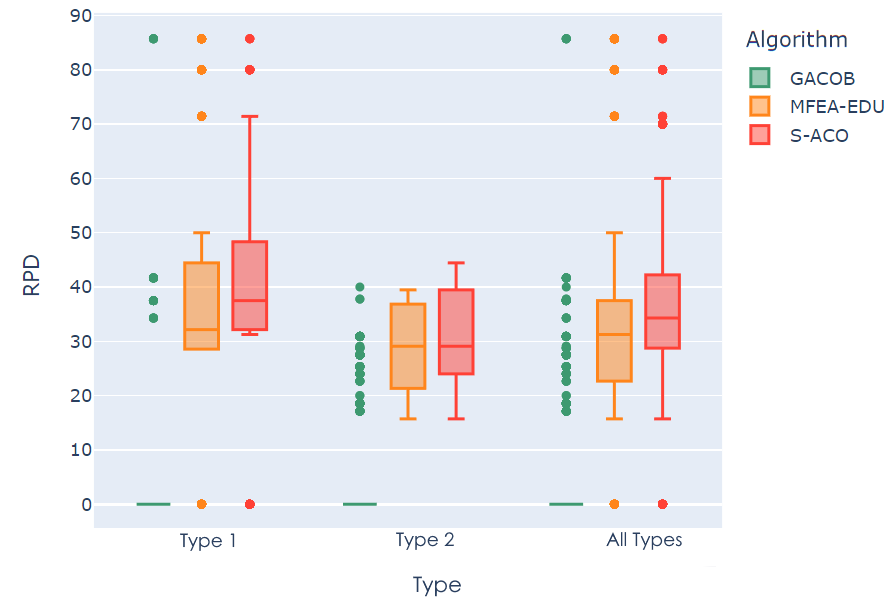
\includegraphics[scale=\scalefigure]{Figures/chap 4/RPD_each_set.png}
	\caption{The obtained RPD values of all algorithms}
	\label{fig:rpd}
\end{figure}

\subsection{Analysis quality of the proposed algorithm in comparison with other algorithms}
The experimental results shown in Table~\ref{tab:type_1} and Table~\ref{tab:type_2} have pointed out that \acrshort{gaco} outperforms \acrshort{saco} and \acrshort{mfea-edu} on both the best value, average, and standard deviation in most instances, except small instant Idpc\_10x10x1000. The box and whisker plots of each instance type and the three algorithms (\acrshort{gaco}, \acrshort{mfea-edu}, and \acrshort{saco}) are shown in Figure~\ref{fig:rpd}. Our algorithm finds the best solution every time, which is why the box and whisker plots in Type 1, Type 2, and All Types are reduced to single lines. The average \gls{pi} of \acrshort{gaco} compared to \acrshort{saco}, as shown in Table~\ref{tab:pi}, is 24.6\% in Type 1 and  18.7\% in Type 2. Meanwhile, the percentage for \acrshort{mfea-edu} is 21.0\% in Type 1 and 17.4\% in Type 2. Overall, the proposed \acrshort{gaco} improves \acrshort{mfea-edu}  19.4\% in terms of the average result, and the enormous gap recorded is 44.4\%.

\begin{table}[htbp]
	\centering
	\caption{The PI of \acrshort{gaco} compared to other algorithms}
	\scalebox{0.9}{
		\begin{tabular}{clccccccc}
			\toprule
			\multirow{2}[4]{*}{} & \multicolumn{1}{l}{\multirow{2}[4]{*}{\textbf{Type}}} & \multicolumn{3}{c}{\textbf{GACOB - S-ACO}} & & \multicolumn{3}{c}{\textbf{GACOB - MFEA-EDU}}  \\
			\cmidrule{3-5} \cmidrule{7-9}& & \textbf{MIN PI} & \textbf{AVG PI} & \textbf{MAX PI} & & \textbf{MIN PI} & \textbf{AVG PI} & \textbf{MAX PI} \\
			\midrule
			& Type 1 & -2.6 & 24.6 & 39.1  & & -1.0 & 21.0 & 44.4\\
			& Type 2 & 2.4  & 18.7 & 29.4 & & 0.2 & 17.4 & 28.3 \\
			\midrule
			& All instances & -2.6  & 22.1 & 39.1 & & -1.0 & 19.4 & 44.4 \\
			\bottomrule
		\end{tabular}%
	}
	\label{tab:pi}%
\end{table}%

\begin{table}[htbp]
	\centering
	\caption{The obtained results of all algorithms in Type 1}
	\scalebox{0.9}{
		\begin{tabular}{clccccccccccc}
			\toprule
			\multirow{2}[4]{*}{} & \multicolumn{1}{l}{\multirow{2}[4]{*}{\textbf{Instances}}} & \multicolumn{3}{c}{\textbf{S-ACO}} & & \multicolumn{3}{c}{\textbf{MFEA-EDU}} & & \multicolumn{3}{c}{\textbf{GACOB}}  \\
			\cmidrule{3-5} \cmidrule{7-9} \cmidrule{11-13}& & \textbf{BF} & \textbf{AVG} & \multicolumn{1}{p{2.5em}}{\textbf{STD}} & & \textbf{BF} & \textbf{AVG} & \multicolumn{1}{p{2.5em}}{\textbf{STD}} & & \textbf{BF} & \textbf{AVG} & \multicolumn{1}{p{2.5em}}{\textbf{STD}} \\
			\midrule
			& Idpc\_10x10x1000 & 7  & 7.80  & 2.07 & & 7 & 12.20 & 2.07  & & 7 & \textcolor[rgb]{ 0,  0,  1}{8.00} & 2.27  \\
			& Idpc\_10x20x2713 & 7  & 7.83  & 1.90 & & 12 & 12.00 & 0.00  & & 7 & \textcolor[rgb]{ 1,  0,  0}{7.00} & 0.00 \\
			& Idpc\_10x5x425 & 7  & 7.00  & 0.00 & & 7 & 7.00 & 0.00  & & 7 & \textcolor[rgb]{ 0,  0,  0}{7.00} & 0.00 \\
			& Idpc\_15x15x3375 & 16  & 16.40  & 0.50 & & 10 & 10.00 & 0.00  & & 10 & \textcolor[rgb]{ 0,  0,  0}{10.00} & 0.00 \\
			& Idpc\_15x30x12111 & 10  & 16.43  & 1.30 & & 10 & 10.00 & 0.00  & & 10 & \textcolor[rgb]{ 0,  0,  0}{10.00} & 0.00 \\
			& Idpc\_15x7x1504 & 10  & 13.73  & 4.06 & & 18 & 18.00 & 0.00  & & 10 & \textcolor[rgb]{ 1,  0,  0}{10.00} & 0.00 \\
			& Idpc\_20x10x2492 & 22  & 22.00  & 0.00 & & 22 & 22.00 & 0.00  & & 15 & \textcolor[rgb]{ 1,  0,  0}{15.00} & 0.00 \\
			& Idpc\_20x20x8000 & 21  & 22.07  & 0.83 & & 15 & 15.40 & 1.52  & & 15 & \textcolor[rgb]{ 1,  0,  0}{15.00} & 0.00 \\
			& Idpc\_20x40x26104 & 21  & 22.00  & 0.37 & & 15 & 15.20 & 1.10  & & 15 & \textcolor[rgb]{ 1,  0,  0}{15.00} & 0.00 \\
			& Idpc\_25x12x4817 & 27  & 27.00  & 0.00 & & 27 & 27.00 & 0.00  & & 18 & \textcolor[rgb]{ 1,  0,  0}{18.00} & 0.00 \\
			& Idpc\_25x25x15625 & 26  & 26.90  & 0.31 & & 18 & 24.13 & 3.44  & & 18 & \textcolor[rgb]{ 1,  0,  0}{18.00} & 0.00 \\
			& Idpc\_20x50x57147 & 26  & 26.93  & 0.25 & & 18 & 24.67 & 3.03  & & 18 & \textcolor[rgb]{ 1,  0,  0}{18.00} & 0.00 \\
			& Idpc\_30x15x10025 & 33  & 33.93  & 0.25 & & 33 & 33.00 & 0.00 & & 33 & \textcolor[rgb]{ 1,  0,  0}{33.33} & 0.48 \\
			& Idpc\_30x30x27000 & 32  & 32.73  & 0.45 & & 32 & 32.00 & 0.00 & & 24 & \textcolor[rgb]{ 1,  0,  0}{24.00} & 0.00 \\
			& Idpc\_30x60x89772 & 32  & 32.33  & 0.48 & & 32 & 32.00 & 0.00 & & 24 & \textcolor[rgb]{ 1,  0,  0}{24.00} & 0.00 \\
			& Idpc\_35x17x13934 & 38  & 38.50  & 0.51 & & 38 & 38.00 & 0.00 & & 28 & \textcolor[rgb]{ 1,  0,  0}{28.00} & 0.00 \\
			& Idpc\_35x35x42875 & 37  & 38.47  & 0.82 & & 37 & 37.00 & 0.00 & & 28 & \textcolor[rgb]{ 1,  0,  0}{28.00} & 0.00 \\
			& Idpc\_35x70x123585 & 37  & 37.00  & 0.00 & & 28 & 35.47 & 2.03 & & 28 & \textcolor[rgb]{ 1,  0,  0}{28.00} & 0.00 \\
			& Idpc\_40x20x18485 & 42  & 42.97  & 0.18 & & 42 & 42.00 & 0.00 & & 32 & \textcolor[rgb]{ 1,  0,  0}{32.00} & 0.00 \\
			& Idpc\_40x40x64000 & 42  & 42.00  & 0.00 & & 42 & 42.00 & 0.00 & & 32 & \textcolor[rgb]{ 1,  0,  0}{32.00} & 0.00 \\
			& Idpc\_40x80x130681 & 42  & 42.00  & 0.00 & & 42 & 42.00 & 0.00 & & 32 & \textcolor[rgb]{ 1,  0,  0}{32.00} & 0.00 \\
			& Idpc\_45x22x43769 & 47  & 47.00  & 0.00 & & 47 & 47.00 & 0.00 & & 35 & \textcolor[rgb]{ 1,  0,  0}{37.00} & 4.55 \\
			& Idpc\_45x45x91125 & 47  & 48.93  & 0.37 & & 46 & 46.00 & 0.00 & & 35 & \textcolor[rgb]{ 1,  0,  0}{35.00} & 0.00 \\
			& Idpc\_45x90x322081 & 46  & 46.90  & 0.31 & & 46 & 46.00 & 0.00 & & 35 & \textcolor[rgb]{ 1,  0,  0}{35.00} & 0.00 \\
			\bottomrule
		\end{tabular}
	}
	\label{tab:type_1}%
\end{table}

\begin{table}[htbp]
	\centering
	\caption{The obtained results of all algorithms in Type 2}
	\scalebox{0.9}{
		\begin{tabular}{clccccccccccc}
			\toprule
			\multirow{2}[4]{*}{} & \multicolumn{1}{l}{\multirow{2}[4]{*}{\textbf{Instances}}} & \multicolumn{3}{c}{\textbf{S-ACO}} & & \multicolumn{3}{c}{\textbf{MFEA-EDU}} & & \multicolumn{3}{c}{\textbf{GACOB}}  \\
			\cmidrule{3-5} \cmidrule{7-9} \cmidrule{11-13}& & \textbf{BF} & \textbf{AVG} & \multicolumn{1}{p{2.5em}}{\textbf{STD}} & & \textbf{BF} & \textbf{AVG} & \multicolumn{1}{p{2.5em}}{\textbf{STD}} & & \textbf{BF} & \textbf{AVG} & \multicolumn{1}{p{2.5em}}{\textbf{STD}} \\
			\midrule
			& Idpc\_100x100x1000000 & 103  & 103.03  & 0.18  & & 102 & 102.00 & 0.00  & & 80 & \textcolor[rgb]{ 1,  0,  0}{91.17} & 11.36  \\
			& Idpc\_100x200x2296097 & 102  & 102.00  & 0.00 & & 101 & 101.00 & 0.00  & & 80 & \textcolor[rgb]{ 1,  0,  0}{96.87} & 9.46 \\
			& Idpc\_100x50x461319 & 103  & 103.00  & 0.00 & & 102 & 102.07 & 0.37  & & 80 & \textcolor[rgb]{ 1,  0,  0}{80.00} & 0.00 \\
			& Idpc\_50x100x285357 & 52  & 52.00  & 0.00 & & 52 & 52.00 & 0.00  & & 38 & \textcolor[rgb]{ 1,  0,  0}{38.00} & 0.00 \\
			& Idpc\_50x25x38961 & 53  & 53.00  & 0.00 & & 53 & 53.00 & 0.00  & & 38 & \textcolor[rgb]{ 1,  0,  0}{38.00} & 0.00 \\
			& Idpc\_50x50x125000 & 53  & 53.00  & 0.00 & & 52 & 52.00 & 0.00  & & 38 & \textcolor[rgb]{ 1,  0,  0}{38.00} & 0.00 \\
			& Idpc\_60x120x434337 & 64  & 64.07  & 0.25 & & 61 & 61.00 & 0.00  & & 45 & \textcolor[rgb]{ 1,  0,  0}{45.60} & 3.29 \\
			& Idpc\_60x30x99470 & 62  & 63.93  & 0.37 & & 62 & 62.00 & 0.00  & & 45 & \textcolor[rgb]{ 1,  0,  0}{46.13} & 4.31 \\
			& Idpc\_60x60x216000 & 62  & 63.73  & 0.58 & & 62 & 62.00 & 0.00  & & 45 & \textcolor[rgb]{ 1,  0,  0}{45.00} & 0.00 \\
			& Idpc\_70x140x923343 & 73  & 73.00  & 0.00 & & 72 & 72.00 & 0.00  & & 55 & \textcolor[rgb]{ 1,  0,  0}{66.90} & 7.92 \\
			& Idpc\_70x35x120810 & 72  & 72.97  & 0.18 & & 72 & 72.00 & 0.00  & & 55 & \textcolor[rgb]{ 1,  0,  0}{55.57} & 3.10 \\
			& Idpc\_70x70x343000 & 71  & 72.73  & 0.64 & & 71 & 71.00 & 0.00  & & 55 & \textcolor[rgb]{ 1,  0,  0}{56.07} & 4.06 \\
			& Idpc\_80x160x1490468 & 81  & 81.93 & 0.25 & & 81 & 81.00 & 0.00  & & 70 & \textcolor[rgb]{ 1,  0,  0}{70.00} & 0.00 \\
			& Idpc\_80x40x175762 & 82  & 82.97  & 0.18 & & 82 & 82.00 & 0.00  & & 70 & \textcolor[rgb]{ 1,  0,  0}{70.80} & 3.04 \\
			& Idpc\_80x80x512000 & 82  & 83.87 & 0.43 & & 82 & 82.00 & 0.00  & & 70 & \textcolor[rgb]{ 1,  0,  0}{81.83} & 3.27 \\
			& Idpc\_90x180x1644367 & 92 & 92.00 & 0.00 & & 91 & 91.00 & 0.00  & & 75 & \textcolor[rgb]{ 1,  0,  0}{77.83} & 6.44 \\
			& Idpc\_90x45x260195 & 93 & 93.00 & 0.00 & & 93 & 93.20 & 0.48  & & 75 & \textcolor[rgb]{ 1,  0,  0}{75.00} & 0.00 \\
			& Idpc\_90x90x729000 & 93 & 93.97 & 0.18 & & 91 & 91.00 & 0.00 & & 75 & \textcolor[rgb]{ 1,  0,  0}{87.97} & 8.64 \\
			\bottomrule
		\end{tabular}%
	}
	\label{tab:type_2}%
\end{table}